\documentclass[1p]{elsarticle_modified}
%\bibliographystyle{elsarticle-num}

%\usepackage[colorlinks]{hyperref}
%\usepackage{abbrmath_seonhwa} %\Abb, \Ascr, \Acal ,\Abf, \Afrak
\usepackage{amsfonts}
\usepackage{amssymb}
\usepackage{amsmath}
\usepackage{amsthm}
\usepackage{scalefnt}
\usepackage{amsbsy}
\usepackage{kotex}
\usepackage{caption}
\usepackage{subfig}
\usepackage{color}
\usepackage{graphicx}
\usepackage{xcolor} %% white, black, red, green, blue, cyan, magenta, yellow
\usepackage{float}
\usepackage{setspace}
\usepackage{hyperref}

\usepackage{tikz}
\usetikzlibrary{arrows}

\usepackage{multirow}
\usepackage{array} % fixed length table
\usepackage{hhline}

%%%%%%%%%%%%%%%%%%%%%
\makeatletter
\renewcommand*\env@matrix[1][\arraystretch]{%
	\edef\arraystretch{#1}%
	\hskip -\arraycolsep
	\let\@ifnextchar\new@ifnextchar
	\array{*\c@MaxMatrixCols c}}
\makeatother %https://tex.stackexchange.com/questions/14071/how-can-i-increase-the-line-spacing-in-a-matrix
%%%%%%%%%%%%%%%

\usepackage[normalem]{ulem}

\newcommand{\msout}[1]{\ifmmode\text{\sout{\ensuremath{#1}}}\else\sout{#1}\fi}
%SOURCE: \msout is \stkout macro in https://tex.stackexchange.com/questions/20609/strikeout-in-math-mode

\newcommand{\cancel}[1]{
	\ifmmode
	{\color{red}\msout{#1}}
	\else
	{\color{red}\sout{#1}}
	\fi
}

\newcommand{\add}[1]{
	{\color{blue}\uwave{#1}}
}

\newcommand{\replace}[2]{
	\ifmmode
	{\color{red}\msout{#1}}{\color{blue}\uwave{#2}}
	\else
	{\color{red}\sout{#1}}{\color{blue}\uwave{#2}}
	\fi
}

\newcommand{\Sol}{\mathcal{S}} %segment
\newcommand{\D}{D} %diagram
\newcommand{\A}{\mathcal{A}} %arc


%%%%%%%%%%%%%%%%%%%%%%%%%%%%%5 test

\def\sl{\operatorname{\textup{SL}}(2,\Cbb)}
\def\psl{\operatorname{\textup{PSL}}(2,\Cbb)}
\def\quan{\mkern 1mu \triangleright \mkern 1mu}

\theoremstyle{definition}
\newtheorem{thm}{Theorem}[section]
\newtheorem{prop}[thm]{Proposition}
\newtheorem{lem}[thm]{Lemma}
\newtheorem{ques}[thm]{Question}
\newtheorem{cor}[thm]{Corollary}
\newtheorem{defn}[thm]{Definition}
\newtheorem{exam}[thm]{Example}
\newtheorem{rmk}[thm]{Remark}
\newtheorem{alg}[thm]{Algorithm}

\newcommand{\I}{\sqrt{-1}}
\begin{document}

%\begin{frontmatter}
%
%\title{Boundary parabolic representations of knots up to 8 crossings}
%
%%% Group authors per affiliation:
%\author{Yunhi Cho} 
%\address{Department of Mathematics, University of Seoul, Seoul, Korea}
%\ead{yhcho@uos.ac.kr}
%
%
%\author{Seonhwa Kim} %\fnref{s_kim}}
%\address{Center for Geometry and Physics, Institute for Basic Science, Pohang, 37673, Korea}
%\ead{ryeona17@ibs.re.kr}
%
%\author{Hyuk Kim}
%\address{Department of Mathematical Sciences, Seoul National University, Seoul 08826, Korea}
%\ead{hyukkim@snu.ac.kr}
%
%\author{Seokbeom Yoon}
%\address{Department of Mathematical Sciences, Seoul National University, Seoul, 08826,  Korea}
%\ead{sbyoon15@snu.ac.kr}
%
%\begin{abstract}
%We find all boundary parabolic representation of knots up to 8 crossings.
%
%\end{abstract}
%\begin{keyword}
%    \MSC[2010] 57M25 
%\end{keyword}
%
%\end{frontmatter}

%\linenumbers
%\tableofcontents
%
\newcommand\colored[1]{\textcolor{white}{\rule[-0.35ex]{0.8em}{1.4ex}}\kern-0.8em\color{red} #1}%
%\newcommand\colored[1]{\textcolor{white}{ #1}\kern-2.17ex	\textcolor{white}{ #1}\kern-1.81ex	\textcolor{white}{ #1}\kern-2.15ex\color{red}#1	}

{\Large $\underline{12a_{1108}~(K12a_{1108})}$}

\setlength{\tabcolsep}{10pt}
\renewcommand{\arraystretch}{1.6}
\vspace{1cm}\begin{tabular}{m{100pt}>{\centering\arraybackslash}m{274pt}}
\multirow{5}{120pt}{
	\centering
	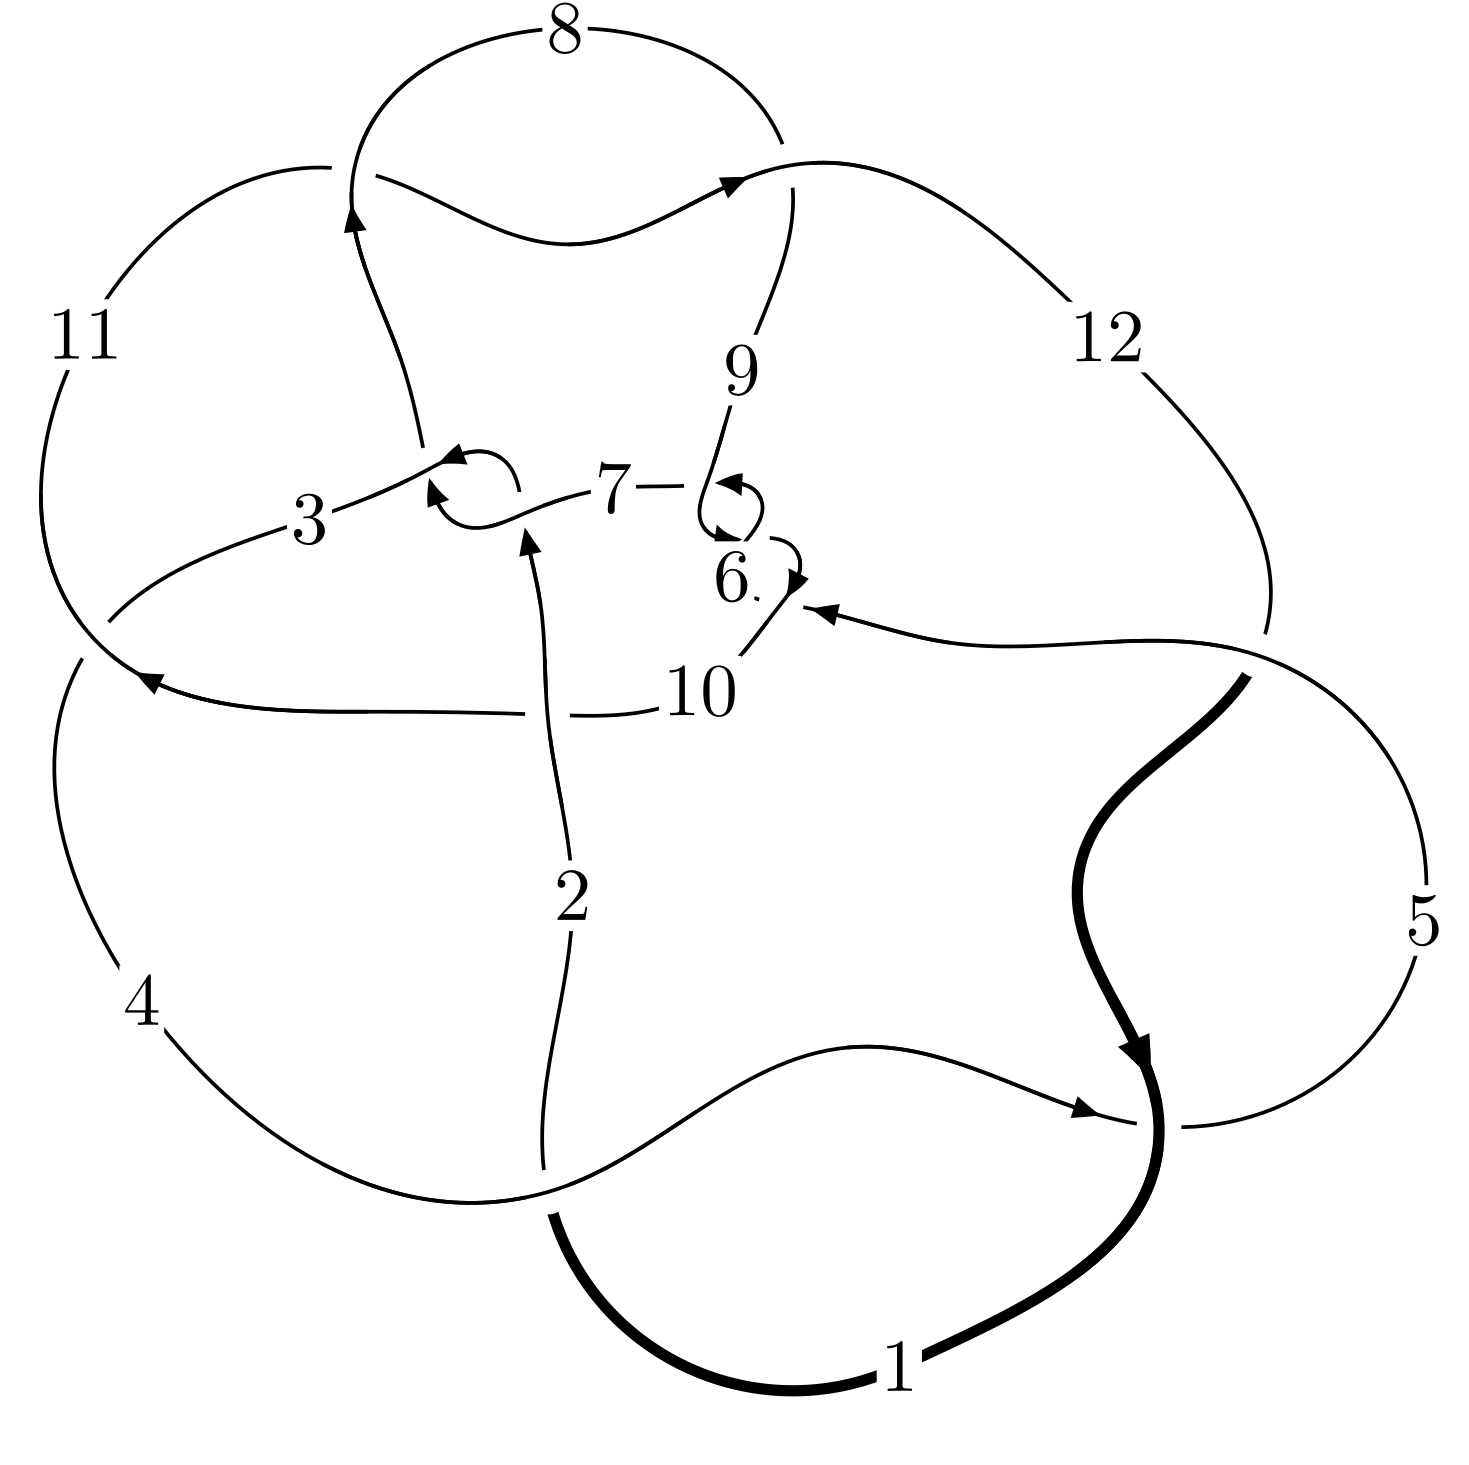
\includegraphics[width=112pt]{../../../GIT/diagram.site/Diagrams/png/1909_12a_1108.png}\\
\ \ \ A knot diagram\footnotemark}&
\allowdisplaybreaks
\textbf{Linearized knot diagam} \\
\cline{2-2}
 &
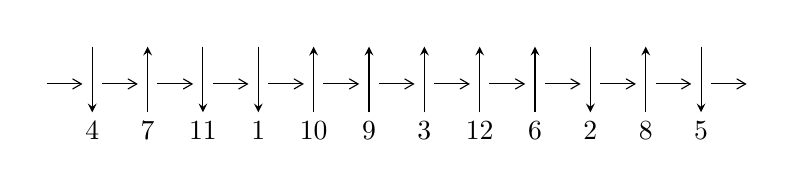
\begin{tikzpicture}[x=20pt, y=17pt]
	% nodes
	\node (C0) at (0, 0) {};
	\node (C1) at (1, 0) {};
	\node (C1U) at (1, +1) {};
	\node (C1D) at (1, -1) {4};

	\node (C2) at (2, 0) {};
	\node (C2U) at (2, +1) {};
	\node (C2D) at (2, -1) {7};

	\node (C3) at (3, 0) {};
	\node (C3U) at (3, +1) {};
	\node (C3D) at (3, -1) {11};

	\node (C4) at (4, 0) {};
	\node (C4U) at (4, +1) {};
	\node (C4D) at (4, -1) {1};

	\node (C5) at (5, 0) {};
	\node (C5U) at (5, +1) {};
	\node (C5D) at (5, -1) {10};

	\node (C6) at (6, 0) {};
	\node (C6U) at (6, +1) {};
	\node (C6D) at (6, -1) {9};

	\node (C7) at (7, 0) {};
	\node (C7U) at (7, +1) {};
	\node (C7D) at (7, -1) {3};

	\node (C8) at (8, 0) {};
	\node (C8U) at (8, +1) {};
	\node (C8D) at (8, -1) {12};

	\node (C9) at (9, 0) {};
	\node (C9U) at (9, +1) {};
	\node (C9D) at (9, -1) {6};

	\node (C10) at (10, 0) {};
	\node (C10U) at (10, +1) {};
	\node (C10D) at (10, -1) {2};

	\node (C11) at (11, 0) {};
	\node (C11U) at (11, +1) {};
	\node (C11D) at (11, -1) {8};

	\node (C12) at (12, 0) {};
	\node (C12U) at (12, +1) {};
	\node (C12D) at (12, -1) {5};
	\node (C13) at (13, 0) {};

	% arrows
	\draw[->,>={angle 60}]
	(C0) edge (C1) (C1) edge (C2) (C2) edge (C3) (C3) edge (C4) (C4) edge (C5) (C5) edge (C6) (C6) edge (C7) (C7) edge (C8) (C8) edge (C9) (C9) edge (C10) (C10) edge (C11) (C11) edge (C12) (C12) edge (C13) ;	\draw[->,>=stealth]
	(C1U) edge (C1D) (C2D) edge (C2U) (C3U) edge (C3D) (C4U) edge (C4D) (C5D) edge (C5U) (C6D) edge (C6U) (C7D) edge (C7U) (C8D) edge (C8U) (C9D) edge (C9U) (C10U) edge (C10D) (C11D) edge (C11U) (C12U) edge (C12D) ;
	\end{tikzpicture} \\
\hhline{~~} \\& 
\textbf{Solving Sequence} \\ \cline{2-2} 
 &
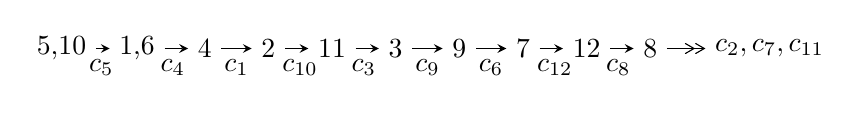
\begin{tikzpicture}[x=23pt, y=7pt]
	% node
	\node (A0) at (-1/8, 0) {5,10};
	\node (A1) at (17/16, 0) {1,6};
	\node (A2) at (17/8, 0) {4};
	\node (A3) at (25/8, 0) {2};
	\node (A4) at (33/8, 0) {11};
	\node (A5) at (41/8, 0) {3};
	\node (A6) at (49/8, 0) {9};
	\node (A7) at (57/8, 0) {7};
	\node (A8) at (65/8, 0) {12};
	\node (A9) at (73/8, 0) {8};
	\node (C1) at (1/2, -1) {$c_{5}$};
	\node (C2) at (13/8, -1) {$c_{4}$};
	\node (C3) at (21/8, -1) {$c_{1}$};
	\node (C4) at (29/8, -1) {$c_{10}$};
	\node (C5) at (37/8, -1) {$c_{3}$};
	\node (C6) at (45/8, -1) {$c_{9}$};
	\node (C7) at (53/8, -1) {$c_{6}$};
	\node (C8) at (61/8, -1) {$c_{12}$};
	\node (C9) at (69/8, -1) {$c_{8}$};
	\node (A10) at (11, 0) {$c_{2},c_{7},c_{11}$};

	% edge
	\draw[->,>=stealth]	
	(A0) edge (A1) (A1) edge (A2) (A2) edge (A3) (A3) edge (A4) (A4) edge (A5) (A5) edge (A6) (A6) edge (A7) (A7) edge (A8) (A8) edge (A9) ;
	\draw[->>,>={angle 60}]	
	(A9) edge (A10);
\end{tikzpicture} \\ 

\end{tabular} \\

\footnotetext{
The image of knot diagram is generated by the software ``\textbf{Draw programme}" developed by Andrew Bartholomew(\url{http://www.layer8.co.uk/maths/draw/index.htm\#Running-draw}), where we modified some parts for our purpose(\url{https://github.com/CATsTAILs/LinksPainter}).
}\phantom \\ \newline 
\centering \textbf{Ideals for irreducible components\footnotemark of $X_{\text{par}}$} 
 
\begin{align*}
I^u_{1}&=\langle 
-8.88369\times10^{219} u^{103}-3.46423\times10^{220} u^{102}+\cdots+1.55368\times10^{220} b+9.10459\times10^{221},\\
\phantom{I^u_{1}}&\phantom{= \langle  }6.55031\times10^{220} u^{103}-1.41928\times10^{221} u^{102}+\cdots+3.57346\times10^{221} a+1.01047\times10^{224},\\
\phantom{I^u_{1}}&\phantom{= \langle  }u^{104}+4 u^{103}+\cdots-4255 u-529\rangle \\
I^u_{2}&=\langle 
u^{25}+4 u^{24}+\cdots+b+3,\;- u^{25}-3 u^{24}+\cdots+a+1,\;u^{27}+3 u^{26}+\cdots+6 u+1\rangle \\
\\
\end{align*}
\raggedright * 2 irreducible components of $\dim_{\mathbb{C}}=0$, with total 131 representations.\\
\footnotetext{All coefficients of polynomials are rational numbers. But the coefficients are sometimes approximated in decimal forms when there is not enough margin.}
\newpage
\renewcommand{\arraystretch}{1}
\centering \section*{I. $I^u_{1}= \langle -8.88\times10^{219} u^{103}-3.46\times10^{220} u^{102}+\cdots+1.55\times10^{220} b+9.10\times10^{221},\;6.55\times10^{220} u^{103}-1.42\times10^{221} u^{102}+\cdots+3.57\times10^{221} a+1.01\times10^{224},\;u^{104}+4 u^{103}+\cdots-4255 u-529 \rangle$}
\flushleft \textbf{(i) Arc colorings}\\
\begin{tabular}{m{7pt} m{180pt} m{7pt} m{180pt} }
\flushright $a_{5}=$&$\begin{pmatrix}1\\0\end{pmatrix}$ \\
\flushright $a_{10}=$&$\begin{pmatrix}0\\u\end{pmatrix}$ \\
\flushright $a_{1}=$&$\begin{pmatrix}-0.183304 u^{103}+0.397174 u^{102}+\cdots-2245.37 u-282.771\\0.571785 u^{103}+2.22970 u^{102}+\cdots-600.028 u-58.6003\end{pmatrix}$ \\
\flushright $a_{6}=$&$\begin{pmatrix}1\\- u^2\end{pmatrix}$ \\
\flushright $a_{4}=$&$\begin{pmatrix}-0.371940 u^{103}-1.83384 u^{102}+\cdots+1047.48 u+109.993\\0.155948 u^{103}+1.00054 u^{102}+\cdots-985.578 u-114.243\end{pmatrix}$ \\
\flushright $a_{2}=$&$\begin{pmatrix}0.386064 u^{103}+1.36986 u^{102}+\cdots-214.929 u-22.7915\\-0.285722 u^{103}-1.16300 u^{102}+\cdots+450.273 u+54.6246\end{pmatrix}$ \\
\flushright $a_{11}=$&$\begin{pmatrix}0.0442397 u^{103}-0.795827 u^{102}+\cdots+2948.61 u+391.066\\0.375507 u^{103}+2.42856 u^{102}+\cdots-3062.77 u-379.760\end{pmatrix}$ \\
\flushright $a_{3}=$&$\begin{pmatrix}0.396800 u^{103}+1.56173 u^{102}+\cdots-404.122 u-41.2529\\-0.283963 u^{103}-1.23407 u^{102}+\cdots+609.778 u+70.8958\end{pmatrix}$ \\
\flushright $a_{9}=$&$\begin{pmatrix}- u\\u^3+u\end{pmatrix}$ \\
\flushright $a_{7}=$&$\begin{pmatrix}u^2+1\\- u^4-2 u^2\end{pmatrix}$ \\
\flushright $a_{12}=$&$\begin{pmatrix}0.388481 u^{103}+2.62687 u^{102}+\cdots-2845.40 u-341.371\\0.571785 u^{103}+2.22970 u^{102}+\cdots-600.028 u-58.6003\end{pmatrix}$ \\
\flushright $a_{8}=$&$\begin{pmatrix}0.201012 u^{103}+1.99070 u^{102}+\cdots-3254.17 u-404.502\\0.251586 u^{103}+0.498810 u^{102}+\cdots+1127.65 u+152.910\end{pmatrix}$\\&\end{tabular}
\flushleft \textbf{(ii) Obstruction class $= -1$}\\~\\
\flushleft \textbf{(iii) Cusp Shapes $= -2.72322 u^{103}-10.0804 u^{102}+\cdots+428.095 u-67.4251$}\\~\\
\newpage\renewcommand{\arraystretch}{1}
\flushleft \textbf{(iv) u-Polynomials at the component}\newline \\
\begin{tabular}{m{50pt}|m{274pt}}
Crossings & \hspace{64pt}u-Polynomials at each crossing \\
\hline $$\begin{aligned}c_{1},c_{4},c_{12}\end{aligned}$$&$\begin{aligned}
&u^{104}-4 u^{103}+\cdots+30 u-4
\end{aligned}$\\
\hline $$\begin{aligned}c_{2},c_{7}\end{aligned}$$&$\begin{aligned}
&u^{104}+u^{103}+\cdots+795 u+2071
\end{aligned}$\\
\hline $$\begin{aligned}c_{3}\end{aligned}$$&$\begin{aligned}
&u^{104}+26 u^{102}+\cdots+8003385 u-1611677
\end{aligned}$\\
\hline $$\begin{aligned}c_{5},c_{6},c_{9}\end{aligned}$$&$\begin{aligned}
&u^{104}+4 u^{103}+\cdots-4255 u-529
\end{aligned}$\\
\hline $$\begin{aligned}c_{8},c_{11}\end{aligned}$$&$\begin{aligned}
&u^{104}-42 u^{102}+\cdots-17433 u+11887
\end{aligned}$\\
\hline $$\begin{aligned}c_{10}\end{aligned}$$&$\begin{aligned}
&u^{104}+7 u^{103}+\cdots+3018333 u-281591
\end{aligned}$\\
\hline
\end{tabular}\\~\\
\newpage\renewcommand{\arraystretch}{1}
\flushleft \textbf{(v) Riley Polynomials at the component}\newline \\
\begin{tabular}{m{50pt}|m{274pt}}
Crossings & \hspace{64pt}Riley Polynomials at each crossing \\
\hline $$\begin{aligned}c_{1},c_{4},c_{12}\end{aligned}$$&$\begin{aligned}
&y^{104}+106 y^{103}+\cdots-1084 y+16
\end{aligned}$\\
\hline $$\begin{aligned}c_{2},c_{7}\end{aligned}$$&$\begin{aligned}
&y^{104}-71 y^{103}+\cdots-59982743 y+4289041
\end{aligned}$\\
\hline $$\begin{aligned}c_{3}\end{aligned}$$&$\begin{aligned}
&y^{104}+52 y^{103}+\cdots+80900979801019 y+2597502752329
\end{aligned}$\\
\hline $$\begin{aligned}c_{5},c_{6},c_{9}\end{aligned}$$&$\begin{aligned}
&y^{104}+96 y^{103}+\cdots-1564253 y+279841
\end{aligned}$\\
\hline $$\begin{aligned}c_{8},c_{11}\end{aligned}$$&$\begin{aligned}
&y^{104}-84 y^{103}+\cdots-776703027 y+141300769
\end{aligned}$\\
\hline $$\begin{aligned}c_{10}\end{aligned}$$&$\begin{aligned}
&y^{104}+23 y^{103}+\cdots-1658049684805 y+79293491281
\end{aligned}$\\
\hline
\end{tabular}\\~\\
\newpage\flushleft \textbf{(vi) Complex Volumes and Cusp Shapes}
$$\begin{array}{c|c|c}  
\text{Solutions to }I^u_{1}& \I (\text{vol} + \sqrt{-1}CS) & \text{Cusp shape}\\
 \hline 
\begin{aligned}
u &= \phantom{-}0.998404 + 0.066441 I \\
a &= \phantom{-}0.40664 + 2.25976 I \\
b &= \phantom{-}0.024542 - 1.362530 I\end{aligned}
 & \phantom{-}5.41766 + 0.40969 I & \phantom{-0.000000 } 0 \\ \hline\begin{aligned}
u &= \phantom{-}0.998404 - 0.066441 I \\
a &= \phantom{-}0.40664 - 2.25976 I \\
b &= \phantom{-}0.024542 + 1.362530 I\end{aligned}
 & \phantom{-}5.41766 - 0.40969 I & \phantom{-0.000000 } 0 \\ \hline\begin{aligned}
u &= -0.969486 + 0.282556 I \\
a &= \phantom{-}0.04918 - 2.23361 I \\
b &= -0.149167 + 1.248050 I\end{aligned}
 & \phantom{-}5.89794 + 2.79943 I & \phantom{-0.000000 } 0 \\ \hline\begin{aligned}
u &= -0.969486 - 0.282556 I \\
a &= \phantom{-}0.04918 + 2.23361 I \\
b &= -0.149167 - 1.248050 I\end{aligned}
 & \phantom{-}5.89794 - 2.79943 I & \phantom{-0.000000 } 0 \\ \hline\begin{aligned}
u &= \phantom{-}0.872225 + 0.386027 I \\
a &= -0.63402 - 1.93115 I \\
b &= -0.23272 + 1.53537 I\end{aligned}
 & \phantom{-}8.77117 + 6.22222 I & \phantom{-0.000000 } 0 \\ \hline\begin{aligned}
u &= \phantom{-}0.872225 - 0.386027 I \\
a &= -0.63402 + 1.93115 I \\
b &= -0.23272 - 1.53537 I\end{aligned}
 & \phantom{-}8.77117 - 6.22222 I & \phantom{-0.000000 } 0 \\ \hline\begin{aligned}
u &= -0.633735 + 0.860627 I \\
a &= -0.285219 - 0.398896 I \\
b &= \phantom{-}0.427811 - 0.402352 I\end{aligned}
 & \phantom{-}4.64761 + 3.38555 I & \phantom{-0.000000 } 0 \\ \hline\begin{aligned}
u &= -0.633735 - 0.860627 I \\
a &= -0.285219 + 0.398896 I \\
b &= \phantom{-}0.427811 + 0.402352 I\end{aligned}
 & \phantom{-}4.64761 - 3.38555 I & \phantom{-0.000000 } 0 \\ \hline\begin{aligned}
u &= \phantom{-}0.073852 + 1.066990 I \\
a &= \phantom{-}2.00678 - 0.01381 I \\
b &= \phantom{-}0.305195 - 1.270380 I\end{aligned}
 & \phantom{-}6.26427 + 4.42302 I & \phantom{-0.000000 } 0 \\ \hline\begin{aligned}
u &= \phantom{-}0.073852 - 1.066990 I \\
a &= \phantom{-}2.00678 + 0.01381 I \\
b &= \phantom{-}0.305195 + 1.270380 I\end{aligned}
 & \phantom{-}6.26427 - 4.42302 I & \phantom{-0.000000 } 0\\
 \hline 
 \end{array}$$\newpage$$\begin{array}{c|c|c}  
\text{Solutions to }I^u_{1}& \I (\text{vol} + \sqrt{-1}CS) & \text{Cusp shape}\\
 \hline 
\begin{aligned}
u &= -1.023460 + 0.312641 I \\
a &= \phantom{-}0.53307 - 2.07864 I \\
b &= \phantom{-}0.25526 + 1.51975 I\end{aligned}
 & \phantom{-}12.9579 - 11.9173 I & \phantom{-0.000000 } 0 \\ \hline\begin{aligned}
u &= -1.023460 - 0.312641 I \\
a &= \phantom{-}0.53307 + 2.07864 I \\
b &= \phantom{-}0.25526 - 1.51975 I\end{aligned}
 & \phantom{-}12.9579 + 11.9173 I & \phantom{-0.000000 } 0 \\ \hline\begin{aligned}
u &= -0.928373\phantom{ +0.000000I} \\
a &= \phantom{-}0.323165\phantom{ +0.000000I} \\
b &= -0.614916\phantom{ +0.000000I}\end{aligned}
 & \phantom{-}2.21584\phantom{ +0.000000I} & \phantom{-0.000000 } 0 \\ \hline\begin{aligned}
u &= \phantom{-}0.785609 + 0.754829 I \\
a &= \phantom{-}0.81012 + 1.33339 I \\
b &= -0.08988 - 1.48205 I\end{aligned}
 & \phantom{-}7.69660 - 0.76643 I & \phantom{-0.000000 } 0 \\ \hline\begin{aligned}
u &= \phantom{-}0.785609 - 0.754829 I \\
a &= \phantom{-}0.81012 - 1.33339 I \\
b &= -0.08988 + 1.48205 I\end{aligned}
 & \phantom{-}7.69660 + 0.76643 I & \phantom{-0.000000 } 0 \\ \hline\begin{aligned}
u &= -0.822823 + 0.300153 I \\
a &= -0.136303 - 0.641555 I \\
b &= \phantom{-}0.729313 + 0.530280 I\end{aligned}
 & \phantom{-}6.29249 - 8.31502 I & \phantom{-0.000000 } 0 \\ \hline\begin{aligned}
u &= -0.822823 - 0.300153 I \\
a &= -0.136303 + 0.641555 I \\
b &= \phantom{-}0.729313 - 0.530280 I\end{aligned}
 & \phantom{-}6.29249 + 8.31502 I & \phantom{-0.000000 } 0 \\ \hline\begin{aligned}
u &= \phantom{-}0.651115 + 0.577237 I \\
a &= -0.40122 - 2.24284 I \\
b &= \phantom{-}0.169860 + 1.381650 I\end{aligned}
 & \phantom{-}7.11747 - 1.89662 I & \phantom{-0.000000 } 0 \\ \hline\begin{aligned}
u &= \phantom{-}0.651115 - 0.577237 I \\
a &= -0.40122 + 2.24284 I \\
b &= \phantom{-}0.169860 - 1.381650 I\end{aligned}
 & \phantom{-}7.11747 + 1.89662 I & \phantom{-0.000000 } 0 \\ \hline\begin{aligned}
u &= -0.181205 + 1.139620 I \\
a &= -0.111011 + 0.759565 I \\
b &= \phantom{-}0.14074 - 1.71793 I\end{aligned}
 & \phantom{-}10.52570 - 2.57968 I & \phantom{-0.000000 } 0\\
 \hline 
 \end{array}$$\newpage$$\begin{array}{c|c|c}  
\text{Solutions to }I^u_{1}& \I (\text{vol} + \sqrt{-1}CS) & \text{Cusp shape}\\
 \hline 
\begin{aligned}
u &= -0.181205 - 1.139620 I \\
a &= -0.111011 - 0.759565 I \\
b &= \phantom{-}0.14074 + 1.71793 I\end{aligned}
 & \phantom{-}10.52570 + 2.57968 I & \phantom{-0.000000 } 0 \\ \hline\begin{aligned}
u &= \phantom{-}0.082428 + 1.155290 I \\
a &= -2.21153 - 1.42249 I \\
b &= -0.027261 + 1.335620 I\end{aligned}
 & \phantom{-}5.81144 - 3.37082 I & \phantom{-0.000000 } 0 \\ \hline\begin{aligned}
u &= \phantom{-}0.082428 - 1.155290 I \\
a &= -2.21153 + 1.42249 I \\
b &= -0.027261 - 1.335620 I\end{aligned}
 & \phantom{-}5.81144 + 3.37082 I & \phantom{-0.000000 } 0 \\ \hline\begin{aligned}
u &= -0.098594 + 1.227330 I \\
a &= \phantom{-}0.06407 - 1.94244 I \\
b &= -0.01603 + 1.65998 I\end{aligned}
 & \phantom{-}9.41869 + 0.21611 I & \phantom{-0.000000 } 0 \\ \hline\begin{aligned}
u &= -0.098594 - 1.227330 I \\
a &= \phantom{-}0.06407 + 1.94244 I \\
b &= -0.01603 - 1.65998 I\end{aligned}
 & \phantom{-}9.41869 - 0.21611 I & \phantom{-0.000000 } 0 \\ \hline\begin{aligned}
u &= -0.196901 + 1.225630 I \\
a &= \phantom{-}1.163310 - 0.102328 I \\
b &= \phantom{-}0.834652 + 0.152457 I\end{aligned}
 & \phantom{-}2.82236 + 0.39547 I & \phantom{-0.000000 } 0 \\ \hline\begin{aligned}
u &= -0.196901 - 1.225630 I \\
a &= \phantom{-}1.163310 + 0.102328 I \\
b &= \phantom{-}0.834652 - 0.152457 I\end{aligned}
 & \phantom{-}2.82236 - 0.39547 I & \phantom{-0.000000 } 0 \\ \hline\begin{aligned}
u &= \phantom{-}0.136309 + 1.256230 I \\
a &= -0.543584 + 0.051104 I \\
b &= -0.796096 - 1.079340 I\end{aligned}
 & -1.41379 - 0.49702 I & \phantom{-0.000000 } 0 \\ \hline\begin{aligned}
u &= \phantom{-}0.136309 - 1.256230 I \\
a &= -0.543584 - 0.051104 I \\
b &= -0.796096 + 1.079340 I\end{aligned}
 & -1.41379 + 0.49702 I & \phantom{-0.000000 } 0 \\ \hline\begin{aligned}
u &= \phantom{-}0.571816 + 0.454044 I \\
a &= -0.216301 - 0.296006 I \\
b &= \phantom{-}0.443926 + 0.330981 I\end{aligned}
 & \phantom{-}1.77754 + 0.38509 I & \phantom{-}4.38443 + 0.48534 I\\
 \hline 
 \end{array}$$\newpage$$\begin{array}{c|c|c}  
\text{Solutions to }I^u_{1}& \I (\text{vol} + \sqrt{-1}CS) & \text{Cusp shape}\\
 \hline 
\begin{aligned}
u &= \phantom{-}0.571816 - 0.454044 I \\
a &= -0.216301 + 0.296006 I \\
b &= \phantom{-}0.443926 - 0.330981 I\end{aligned}
 & \phantom{-}1.77754 - 0.38509 I & \phantom{-}4.38443 - 0.48534 I \\ \hline\begin{aligned}
u &= \phantom{-}0.667908 + 0.292392 I \\
a &= \phantom{-}0.96415 + 3.27127 I \\
b &= \phantom{-}0.15855 - 1.46104 I\end{aligned}
 & \phantom{-}7.79155 + 5.85095 I & \phantom{-}9.05721 - 6.34260 I \\ \hline\begin{aligned}
u &= \phantom{-}0.667908 - 0.292392 I \\
a &= \phantom{-}0.96415 - 3.27127 I \\
b &= \phantom{-}0.15855 + 1.46104 I\end{aligned}
 & \phantom{-}7.79155 - 5.85095 I & \phantom{-}9.05721 + 6.34260 I \\ \hline\begin{aligned}
u &= \phantom{-}0.573518 + 0.444519 I \\
a &= \phantom{-}0.217991 + 1.214100 I \\
b &= \phantom{-}0.503464 - 0.394630 I\end{aligned}
 & \phantom{-}1.77117 + 3.47379 I & \phantom{-}4.30454 - 8.11372 I \\ \hline\begin{aligned}
u &= \phantom{-}0.573518 - 0.444519 I \\
a &= \phantom{-}0.217991 - 1.214100 I \\
b &= \phantom{-}0.503464 + 0.394630 I\end{aligned}
 & \phantom{-}1.77117 - 3.47379 I & \phantom{-}4.30454 + 8.11372 I \\ \hline\begin{aligned}
u &= -0.130265 + 1.284020 I \\
a &= -1.66242 - 0.57082 I \\
b &= -0.161378 - 0.095670 I\end{aligned}
 & \phantom{-}1.67702 - 4.00381 I & \phantom{-0.000000 } 0 \\ \hline\begin{aligned}
u &= -0.130265 - 1.284020 I \\
a &= -1.66242 + 0.57082 I \\
b &= -0.161378 + 0.095670 I\end{aligned}
 & \phantom{-}1.67702 + 4.00381 I & \phantom{-0.000000 } 0 \\ \hline\begin{aligned}
u &= -0.672561 + 0.216268 I \\
a &= \phantom{-}1.00368 - 1.90578 I \\
b &= \phantom{-}0.25153 + 1.56236 I\end{aligned}
 & \phantom{-}13.11990 - 0.50623 I & \phantom{-}12.21127 + 0.97407 I \\ \hline\begin{aligned}
u &= -0.672561 - 0.216268 I \\
a &= \phantom{-}1.00368 + 1.90578 I \\
b &= \phantom{-}0.25153 - 1.56236 I\end{aligned}
 & \phantom{-}13.11990 + 0.50623 I & \phantom{-}12.21127 - 0.97407 I \\ \hline\begin{aligned}
u &= -0.172810 + 1.289970 I \\
a &= \phantom{-}1.03528 - 1.11652 I \\
b &= \phantom{-}0.119702 + 1.332210 I\end{aligned}
 & \phantom{-}0.233186 + 0.396521 I & \phantom{-0.000000 } 0\\
 \hline 
 \end{array}$$\newpage$$\begin{array}{c|c|c}  
\text{Solutions to }I^u_{1}& \I (\text{vol} + \sqrt{-1}CS) & \text{Cusp shape}\\
 \hline 
\begin{aligned}
u &= -0.172810 - 1.289970 I \\
a &= \phantom{-}1.03528 + 1.11652 I \\
b &= \phantom{-}0.119702 - 1.332210 I\end{aligned}
 & \phantom{-}0.233186 - 0.396521 I & \phantom{-0.000000 } 0 \\ \hline\begin{aligned}
u &= \phantom{-}0.671616\phantom{ +0.000000I} \\
a &= \phantom{-}0.393968\phantom{ +0.000000I} \\
b &= \phantom{-}0.121223\phantom{ +0.000000I}\end{aligned}
 & \phantom{-}1.05986\phantom{ +0.000000I} & \phantom{-}13.1460\phantom{ +0.000000I} \\ \hline\begin{aligned}
u &= -0.207093 + 1.327860 I \\
a &= -1.29131 + 1.11059 I \\
b &= -0.29956 - 1.47499 I\end{aligned}
 & -0.26646 - 5.70650 I & \phantom{-0.000000 } 0 \\ \hline\begin{aligned}
u &= -0.207093 - 1.327860 I \\
a &= -1.29131 - 1.11059 I \\
b &= -0.29956 + 1.47499 I\end{aligned}
 & -0.26646 + 5.70650 I & \phantom{-0.000000 } 0 \\ \hline\begin{aligned}
u &= -0.810446 + 1.082160 I \\
a &= -0.518297 + 1.276570 I \\
b &= \phantom{-}0.16861 - 1.46801 I\end{aligned}
 & \phantom{-}10.77610 + 5.67331 I & \phantom{-0.000000 } 0 \\ \hline\begin{aligned}
u &= -0.810446 - 1.082160 I \\
a &= -0.518297 - 1.276570 I \\
b &= \phantom{-}0.16861 + 1.46801 I\end{aligned}
 & \phantom{-}10.77610 - 5.67331 I & \phantom{-0.000000 } 0 \\ \hline\begin{aligned}
u &= -0.250365 + 1.338370 I \\
a &= \phantom{-}0.281599 + 0.064221 I \\
b &= \phantom{-}0.862834 - 0.787889 I\end{aligned}
 & \phantom{-}1.63639 - 6.53052 I & \phantom{-0.000000 } 0 \\ \hline\begin{aligned}
u &= -0.250365 - 1.338370 I \\
a &= \phantom{-}0.281599 - 0.064221 I \\
b &= \phantom{-}0.862834 + 0.787889 I\end{aligned}
 & \phantom{-}1.63639 + 6.53052 I & \phantom{-0.000000 } 0 \\ \hline\begin{aligned}
u &= \phantom{-}0.393489 + 1.303500 I \\
a &= -0.68596 - 1.41890 I \\
b &= -0.14152 + 1.43341 I\end{aligned}
 & \phantom{-}1.40965 + 4.51412 I & \phantom{-0.000000 } 0 \\ \hline\begin{aligned}
u &= \phantom{-}0.393489 - 1.303500 I \\
a &= -0.68596 + 1.41890 I \\
b &= -0.14152 - 1.43341 I\end{aligned}
 & \phantom{-}1.40965 - 4.51412 I & \phantom{-0.000000 } 0\\
 \hline 
 \end{array}$$\newpage$$\begin{array}{c|c|c}  
\text{Solutions to }I^u_{1}& \I (\text{vol} + \sqrt{-1}CS) & \text{Cusp shape}\\
 \hline 
\begin{aligned}
u &= \phantom{-}0.539367 + 0.337757 I \\
a &= \phantom{-}0.975272 - 0.257796 I \\
b &= -0.064074 - 0.350230 I\end{aligned}
 & \phantom{-}1.46743 + 0.10661 I & \phantom{-}5.93203 + 0.60348 I \\ \hline\begin{aligned}
u &= \phantom{-}0.539367 - 0.337757 I \\
a &= \phantom{-}0.975272 + 0.257796 I \\
b &= -0.064074 + 0.350230 I\end{aligned}
 & \phantom{-}1.46743 - 0.10661 I & \phantom{-}5.93203 - 0.60348 I \\ \hline\begin{aligned}
u &= -0.625129 + 0.102895 I \\
a &= \phantom{-}0.138815 + 0.941849 I \\
b &= \phantom{-}0.778379 - 0.524859 I\end{aligned}
 & \phantom{-}6.20399 - 3.33840 I & \phantom{-}9.20206 + 2.72693 I \\ \hline\begin{aligned}
u &= -0.625129 - 0.102895 I \\
a &= \phantom{-}0.138815 - 0.941849 I \\
b &= \phantom{-}0.778379 + 0.524859 I\end{aligned}
 & \phantom{-}6.20399 + 3.33840 I & \phantom{-}9.20206 - 2.72693 I \\ \hline\begin{aligned}
u &= -0.072414 + 1.379240 I \\
a &= -0.640172 + 0.519110 I \\
b &= -0.786982 - 0.376868 I\end{aligned}
 & -6.25007 - 1.75695 I & \phantom{-0.000000 } 0 \\ \hline\begin{aligned}
u &= -0.072414 - 1.379240 I \\
a &= -0.640172 - 0.519110 I \\
b &= -0.786982 + 0.376868 I\end{aligned}
 & -6.25007 + 1.75695 I & \phantom{-0.000000 } 0 \\ \hline\begin{aligned}
u &= -0.229091 + 1.365350 I \\
a &= -0.037639 - 0.653313 I \\
b &= -0.382110 + 0.941592 I\end{aligned}
 & \phantom{-}0.278441 - 0.737804 I & \phantom{-0.000000 } 0 \\ \hline\begin{aligned}
u &= -0.229091 - 1.365350 I \\
a &= -0.037639 + 0.653313 I \\
b &= -0.382110 - 0.941592 I\end{aligned}
 & \phantom{-}0.278441 + 0.737804 I & \phantom{-0.000000 } 0 \\ \hline\begin{aligned}
u &= \phantom{-}0.567239 + 0.205735 I \\
a &= -0.064922 - 0.596855 I \\
b &= -0.763362 + 0.623857 I\end{aligned}
 & \phantom{-}1.72979 + 2.71370 I & \phantom{-}8.69800 - 7.54641 I \\ \hline\begin{aligned}
u &= \phantom{-}0.567239 - 0.205735 I \\
a &= -0.064922 + 0.596855 I \\
b &= -0.763362 - 0.623857 I\end{aligned}
 & \phantom{-}1.72979 - 2.71370 I & \phantom{-}8.69800 + 7.54641 I\\
 \hline 
 \end{array}$$\newpage$$\begin{array}{c|c|c}  
\text{Solutions to }I^u_{1}& \I (\text{vol} + \sqrt{-1}CS) & \text{Cusp shape}\\
 \hline 
\begin{aligned}
u &= \phantom{-}0.244641 + 1.378890 I \\
a &= -0.704509 - 0.351277 I \\
b &= -1.005120 + 0.397758 I\end{aligned}
 & -3.32666 + 5.76599 I & \phantom{-0.000000 } 0 \\ \hline\begin{aligned}
u &= \phantom{-}0.244641 - 1.378890 I \\
a &= -0.704509 + 0.351277 I \\
b &= -1.005120 - 0.397758 I\end{aligned}
 & -3.32666 - 5.76599 I & \phantom{-0.000000 } 0 \\ \hline\begin{aligned}
u &= -0.522796 + 1.301600 I \\
a &= -1.18192 + 1.47657 I \\
b &= -0.270766 - 1.344250 I\end{aligned}
 & \phantom{-}2.56525 - 8.31671 I & \phantom{-0.000000 } 0 \\ \hline\begin{aligned}
u &= -0.522796 - 1.301600 I \\
a &= -1.18192 - 1.47657 I \\
b &= -0.270766 + 1.344250 I\end{aligned}
 & \phantom{-}2.56525 + 8.31671 I & \phantom{-0.000000 } 0 \\ \hline\begin{aligned}
u &= -0.386313 + 1.358230 I \\
a &= -0.343760 + 0.501923 I \\
b &= -0.729258 - 0.163103 I\end{aligned}
 & -2.16914 - 4.72705 I & \phantom{-0.000000 } 0 \\ \hline\begin{aligned}
u &= -0.386313 - 1.358230 I \\
a &= -0.343760 - 0.501923 I \\
b &= -0.729258 + 0.163103 I\end{aligned}
 & -2.16914 + 4.72705 I & \phantom{-0.000000 } 0 \\ \hline\begin{aligned}
u &= -0.28742 + 1.39789 I \\
a &= \phantom{-}1.250790 - 0.364112 I \\
b &= \phantom{-}0.36538 + 1.43826 I\end{aligned}
 & \phantom{-}7.95514 - 4.03865 I & \phantom{-0.000000 } 0 \\ \hline\begin{aligned}
u &= -0.28742 - 1.39789 I \\
a &= \phantom{-}1.250790 + 0.364112 I \\
b &= \phantom{-}0.36538 - 1.43826 I\end{aligned}
 & \phantom{-}7.95514 + 4.03865 I & \phantom{-0.000000 } 0 \\ \hline\begin{aligned}
u &= \phantom{-}0.21370 + 1.41327 I \\
a &= \phantom{-}0.605805 + 0.166674 I \\
b &= \phantom{-}0.542202 - 0.063337 I\end{aligned}
 & -4.04218 + 2.97751 I & \phantom{-0.000000 } 0 \\ \hline\begin{aligned}
u &= \phantom{-}0.21370 - 1.41327 I \\
a &= \phantom{-}0.605805 - 0.166674 I \\
b &= \phantom{-}0.542202 + 0.063337 I\end{aligned}
 & -4.04218 - 2.97751 I & \phantom{-0.000000 } 0\\
 \hline 
 \end{array}$$\newpage$$\begin{array}{c|c|c}  
\text{Solutions to }I^u_{1}& \I (\text{vol} + \sqrt{-1}CS) & \text{Cusp shape}\\
 \hline 
\begin{aligned}
u &= -0.21887 + 1.41889 I \\
a &= -1.68782 + 0.11155 I \\
b &= -0.06655 - 1.41986 I\end{aligned}
 & \phantom{-}6.85407 - 4.86950 I & \phantom{-0.000000 } 0 \\ \hline\begin{aligned}
u &= -0.21887 - 1.41889 I \\
a &= -1.68782 - 0.11155 I \\
b &= -0.06655 + 1.41986 I\end{aligned}
 & \phantom{-}6.85407 + 4.86950 I & \phantom{-0.000000 } 0 \\ \hline\begin{aligned}
u &= -0.501834 + 0.255964 I \\
a &= -2.79604 + 1.81261 I \\
b &= \phantom{-}0.00008 - 1.53491 I\end{aligned}
 & \phantom{-}12.29450 - 2.11950 I & \phantom{-}13.9495 + 3.8281 I \\ \hline\begin{aligned}
u &= -0.501834 - 0.255964 I \\
a &= -2.79604 - 1.81261 I \\
b &= \phantom{-}0.00008 + 1.53491 I\end{aligned}
 & \phantom{-}12.29450 + 2.11950 I & \phantom{-}13.9495 - 3.8281 I \\ \hline\begin{aligned}
u &= \phantom{-}0.07061 + 1.43505 I \\
a &= -0.287140 - 0.116310 I \\
b &= -0.445250 + 0.808015 I\end{aligned}
 & -4.94431 + 2.81434 I & \phantom{-0.000000 } 0 \\ \hline\begin{aligned}
u &= \phantom{-}0.07061 - 1.43505 I \\
a &= -0.287140 + 0.116310 I \\
b &= -0.445250 - 0.808015 I\end{aligned}
 & -4.94431 - 2.81434 I & \phantom{-0.000000 } 0 \\ \hline\begin{aligned}
u &= \phantom{-}0.27439 + 1.41169 I \\
a &= \phantom{-}1.35331 + 1.41659 I \\
b &= \phantom{-}0.22053 - 1.52889 I\end{aligned}
 & \phantom{-}2.36733 + 9.32735 I & \phantom{-0.000000 } 0 \\ \hline\begin{aligned}
u &= \phantom{-}0.27439 - 1.41169 I \\
a &= \phantom{-}1.35331 - 1.41659 I \\
b &= \phantom{-}0.22053 + 1.52889 I\end{aligned}
 & \phantom{-}2.36733 - 9.32735 I & \phantom{-0.000000 } 0 \\ \hline\begin{aligned}
u &= \phantom{-}0.01734 + 1.44545 I \\
a &= \phantom{-}0.396386 - 0.751706 I \\
b &= \phantom{-}0.268892 + 1.158060 I\end{aligned}
 & -0.534801 - 0.028205 I & \phantom{-0.000000 } 0 \\ \hline\begin{aligned}
u &= \phantom{-}0.01734 - 1.44545 I \\
a &= \phantom{-}0.396386 + 0.751706 I \\
b &= \phantom{-}0.268892 - 1.158060 I\end{aligned}
 & -0.534801 + 0.028205 I & \phantom{-0.000000 } 0\\
 \hline 
 \end{array}$$\newpage$$\begin{array}{c|c|c}  
\text{Solutions to }I^u_{1}& \I (\text{vol} + \sqrt{-1}CS) & \text{Cusp shape}\\
 \hline 
\begin{aligned}
u &= -0.549662 + 0.041925 I \\
a &= -0.09236 + 3.36928 I \\
b &= -0.153243 - 1.394490 I\end{aligned}
 & \phantom{-}4.09130 - 2.97513 I & \phantom{-}1.12422 + 4.10553 I \\ \hline\begin{aligned}
u &= -0.549662 - 0.041925 I \\
a &= -0.09236 - 3.36928 I \\
b &= -0.153243 + 1.394490 I\end{aligned}
 & \phantom{-}4.09130 + 2.97513 I & \phantom{-}1.12422 - 4.10553 I \\ \hline\begin{aligned}
u &= \phantom{-}0.18947 + 1.45243 I \\
a &= \phantom{-}0.658336 + 0.700750 I \\
b &= \phantom{-}0.615723 - 0.503069 I\end{aligned}
 & -4.33718 + 6.21858 I & \phantom{-0.000000 } 0 \\ \hline\begin{aligned}
u &= \phantom{-}0.18947 - 1.45243 I \\
a &= \phantom{-}0.658336 - 0.700750 I \\
b &= \phantom{-}0.615723 + 0.503069 I\end{aligned}
 & -4.33718 - 6.21858 I & \phantom{-0.000000 } 0 \\ \hline\begin{aligned}
u &= -0.33054 + 1.42798 I \\
a &= \phantom{-}0.616003 - 0.560579 I \\
b &= \phantom{-}0.920195 + 0.479120 I\end{aligned}
 & \phantom{-}0.79859 - 12.47880 I & \phantom{-0.000000 } 0 \\ \hline\begin{aligned}
u &= -0.33054 - 1.42798 I \\
a &= \phantom{-}0.616003 + 0.560579 I \\
b &= \phantom{-}0.920195 - 0.479120 I\end{aligned}
 & \phantom{-}0.79859 + 12.47880 I & \phantom{-0.000000 } 0 \\ \hline\begin{aligned}
u &= \phantom{-}0.06538 + 1.47185 I \\
a &= \phantom{-}0.361525 - 0.221663 I \\
b &= \phantom{-}0.461071 + 0.284534 I\end{aligned}
 & -4.56537 + 2.56676 I & \phantom{-0.000000 } 0 \\ \hline\begin{aligned}
u &= \phantom{-}0.06538 - 1.47185 I \\
a &= \phantom{-}0.361525 + 0.221663 I \\
b &= \phantom{-}0.461071 - 0.284534 I\end{aligned}
 & -4.56537 - 2.56676 I & \phantom{-0.000000 } 0 \\ \hline\begin{aligned}
u &= \phantom{-}0.39903 + 1.42674 I \\
a &= \phantom{-}1.17849 + 1.06086 I \\
b &= \phantom{-}0.171298 - 1.352080 I\end{aligned}
 & \phantom{-}0.49101 + 5.48323 I & \phantom{-0.000000 } 0 \\ \hline\begin{aligned}
u &= \phantom{-}0.39903 - 1.42674 I \\
a &= \phantom{-}1.17849 - 1.06086 I \\
b &= \phantom{-}0.171298 + 1.352080 I\end{aligned}
 & \phantom{-}0.49101 - 5.48323 I & \phantom{-0.000000 } 0\\
 \hline 
 \end{array}$$\newpage$$\begin{array}{c|c|c}  
\text{Solutions to }I^u_{1}& \I (\text{vol} + \sqrt{-1}CS) & \text{Cusp shape}\\
 \hline 
\begin{aligned}
u &= -0.472827 + 0.144736 I \\
a &= -1.58765 - 2.63391 I \\
b &= -0.026338 + 0.558642 I\end{aligned}
 & \phantom{-}5.26654 + 1.96738 I & \phantom{-}14.2458 - 2.6393 I \\ \hline\begin{aligned}
u &= -0.472827 - 0.144736 I \\
a &= -1.58765 + 2.63391 I \\
b &= -0.026338 - 0.558642 I\end{aligned}
 & \phantom{-}5.26654 - 1.96738 I & \phantom{-}14.2458 + 2.6393 I \\ \hline\begin{aligned}
u &= \phantom{-}0.15160 + 1.50309 I \\
a &= \phantom{-}0.023024 - 0.305139 I \\
b &= -0.070230 + 0.432947 I\end{aligned}
 & -4.71084 + 2.85923 I & \phantom{-0.000000 } 0 \\ \hline\begin{aligned}
u &= \phantom{-}0.15160 - 1.50309 I \\
a &= \phantom{-}0.023024 + 0.305139 I \\
b &= -0.070230 - 0.432947 I\end{aligned}
 & -4.71084 - 2.85923 I & \phantom{-0.000000 } 0 \\ \hline\begin{aligned}
u &= \phantom{-}0.35014 + 1.47046 I \\
a &= -1.130810 - 0.831992 I \\
b &= -0.36239 + 1.51575 I\end{aligned}
 & \phantom{-}2.85832 + 10.65370 I & \phantom{-0.000000 } 0 \\ \hline\begin{aligned}
u &= \phantom{-}0.35014 - 1.47046 I \\
a &= -1.130810 + 0.831992 I \\
b &= -0.36239 - 1.51575 I\end{aligned}
 & \phantom{-}2.85832 - 10.65370 I & \phantom{-0.000000 } 0 \\ \hline\begin{aligned}
u &= -0.41431 + 1.47342 I \\
a &= \phantom{-}1.23289 - 1.08392 I \\
b &= \phantom{-}0.33859 + 1.53104 I\end{aligned}
 & \phantom{-}7.2848 - 17.0538 I & \phantom{-0.000000 } 0 \\ \hline\begin{aligned}
u &= -0.41431 - 1.47342 I \\
a &= \phantom{-}1.23289 + 1.08392 I \\
b &= \phantom{-}0.33859 - 1.53104 I\end{aligned}
 & \phantom{-}7.2848 + 17.0538 I & \phantom{-0.000000 } 0 \\ \hline\begin{aligned}
u &= \phantom{-}0.113165 + 0.423487 I \\
a &= \phantom{-}0.246557 - 0.386479 I \\
b &= -0.306576 + 0.975377 I\end{aligned}
 & \phantom{-}1.08545 + 2.15056 I & -3.09530 - 5.75751 I \\ \hline\begin{aligned}
u &= \phantom{-}0.113165 - 0.423487 I \\
a &= \phantom{-}0.246557 + 0.386479 I \\
b &= -0.306576 - 0.975377 I\end{aligned}
 & \phantom{-}1.08545 - 2.15056 I & -3.09530 + 5.75751 I\\
 \hline 
 \end{array}$$\newpage$$\begin{array}{c|c|c}  
\text{Solutions to }I^u_{1}& \I (\text{vol} + \sqrt{-1}CS) & \text{Cusp shape}\\
 \hline 
\begin{aligned}
u &= -0.227567 + 0.261070 I \\
a &= \phantom{-}0.20134 + 1.41758 I \\
b &= -0.504243 - 0.205514 I\end{aligned}
 & -1.043770 - 0.672454 I & -5.80489 + 2.84262 I \\ \hline\begin{aligned}
u &= -0.227567 - 0.261070 I \\
a &= \phantom{-}0.20134 - 1.41758 I \\
b &= -0.504243 + 0.205514 I\end{aligned}
 & -1.043770 + 0.672454 I & -5.80489 - 2.84262 I \\ \hline\begin{aligned}
u &= \phantom{-}0.13415 + 1.72704 I \\
a &= \phantom{-}0.292858 + 0.442501 I \\
b &= \phantom{-}0.018613 - 1.343400 I\end{aligned}
 & -1.07790 + 3.06653 I & \phantom{-0.000000 } 0 \\ \hline\begin{aligned}
u &= \phantom{-}0.13415 - 1.72704 I \\
a &= \phantom{-}0.292858 - 0.442501 I \\
b &= \phantom{-}0.018613 + 1.343400 I\end{aligned}
 & -1.07790 - 3.06653 I & \phantom{-0.000000 } 0\\
 \hline 
 \end{array}$$\newpage\newpage\renewcommand{\arraystretch}{1}
\centering \section*{II. $I^u_{2}= \langle u^{25}+4 u^{24}+\cdots+b+3,\;- u^{25}-3 u^{24}+\cdots+a+1,\;u^{27}+3 u^{26}+\cdots+6 u+1 \rangle$}
\flushleft \textbf{(i) Arc colorings}\\
\begin{tabular}{m{7pt} m{180pt} m{7pt} m{180pt} }
\flushright $a_{5}=$&$\begin{pmatrix}1\\0\end{pmatrix}$ \\
\flushright $a_{10}=$&$\begin{pmatrix}0\\u\end{pmatrix}$ \\
\flushright $a_{1}=$&$\begin{pmatrix}u^{25}+3 u^{24}+\cdots+4 u-1\\- u^{25}-4 u^{24}+\cdots-15 u-3\end{pmatrix}$ \\
\flushright $a_{6}=$&$\begin{pmatrix}1\\- u^2\end{pmatrix}$ \\
\flushright $a_{4}=$&$\begin{pmatrix}-3 u^{26}-9 u^{25}+\cdots-16 u-2\\u^{26}+6 u^{25}+\cdots+9 u+2\end{pmatrix}$ \\
\flushright $a_{2}=$&$\begin{pmatrix}- u^{26}-6 u^{25}+\cdots-5 u-1\\-3 u^{26}-4 u^{25}+\cdots+21 u+4\end{pmatrix}$ \\
\flushright $a_{11}=$&$\begin{pmatrix}- u^{26}-5 u^{25}+\cdots-7 u-1\\7 u^{25}+21 u^{24}+\cdots+38 u+6\end{pmatrix}$ \\
\flushright $a_{3}=$&$\begin{pmatrix}-2 u^{26}-9 u^{25}+\cdots-13 u-2\\5 u^{25}+16 u^{24}+\cdots+23 u+4\end{pmatrix}$ \\
\flushright $a_{9}=$&$\begin{pmatrix}- u\\u^3+u\end{pmatrix}$ \\
\flushright $a_{7}=$&$\begin{pmatrix}u^2+1\\- u^4-2 u^2\end{pmatrix}$ \\
\flushright $a_{12}=$&$\begin{pmatrix}- u^{24}-3 u^{23}+\cdots-11 u-4\\- u^{25}-4 u^{24}+\cdots-15 u-3\end{pmatrix}$ \\
\flushright $a_{8}=$&$\begin{pmatrix}u^{26}+4 u^{25}+\cdots+17 u+5\\u^{26}+u^{25}+\cdots+5 u+1\end{pmatrix}$\\&\end{tabular}
\flushleft \textbf{(ii) Obstruction class $= 1$}\\~\\
\flushleft \textbf{(iii) Cusp Shapes $= 5 u^{25}+13 u^{24}+85 u^{23}+182 u^{22}+610 u^{21}+1102 u^{20}+2453 u^{19}+3799 u^{18}+6173 u^{17}+8267 u^{16}+10319 u^{15}+11931 u^{14}+12010 u^{13}+11760 u^{12}+10241 u^{11}+8170 u^{10}+6609 u^9+4250 u^8+3054 u^7+1807 u^6+882 u^5+599 u^4+180 u^3+103 u^2+29 u+14$}\\~\\
\newpage\renewcommand{\arraystretch}{1}
\flushleft \textbf{(iv) u-Polynomials at the component}\newline \\
\begin{tabular}{m{50pt}|m{274pt}}
Crossings & \hspace{64pt}u-Polynomials at each crossing \\
\hline $$\begin{aligned}c_{1},c_{12}\end{aligned}$$&$\begin{aligned}
&u^{27}-3 u^{26}+\cdots+2 u-1
\end{aligned}$\\
\hline $$\begin{aligned}c_{2}\end{aligned}$$&$\begin{aligned}
&u^{27}-9 u^{25}+\cdots-8 u^2+1
\end{aligned}$\\
\hline $$\begin{aligned}c_{3}\end{aligned}$$&$\begin{aligned}
&u^{27}- u^{26}+\cdots+9 u^2+1
\end{aligned}$\\
\hline $$\begin{aligned}c_{4}\end{aligned}$$&$\begin{aligned}
&u^{27}+3 u^{26}+\cdots+2 u+1
\end{aligned}$\\
\hline $$\begin{aligned}c_{5},c_{6}\end{aligned}$$&$\begin{aligned}
&u^{27}+3 u^{26}+\cdots+6 u+1
\end{aligned}$\\
\hline $$\begin{aligned}c_{7}\end{aligned}$$&$\begin{aligned}
&u^{27}-9 u^{25}+\cdots+8 u^2-1
\end{aligned}$\\
\hline $$\begin{aligned}c_{8}\end{aligned}$$&$\begin{aligned}
&u^{27}-5 u^{26}+\cdots-2 u+1
\end{aligned}$\\
\hline $$\begin{aligned}c_{9}\end{aligned}$$&$\begin{aligned}
&u^{27}-3 u^{26}+\cdots+6 u-1
\end{aligned}$\\
\hline $$\begin{aligned}c_{10}\end{aligned}$$&$\begin{aligned}
&u^{27}-2 u^{24}+\cdots-6 u-1
\end{aligned}$\\
\hline $$\begin{aligned}c_{11}\end{aligned}$$&$\begin{aligned}
&u^{27}+5 u^{26}+\cdots-2 u-1
\end{aligned}$\\
\hline
\end{tabular}\\~\\
\newpage\renewcommand{\arraystretch}{1}
\flushleft \textbf{(v) Riley Polynomials at the component}\newline \\
\begin{tabular}{m{50pt}|m{274pt}}
Crossings & \hspace{64pt}Riley Polynomials at each crossing \\
\hline $$\begin{aligned}c_{1},c_{4},c_{12}\end{aligned}$$&$\begin{aligned}
&y^{27}+31 y^{26}+\cdots-8 y-1
\end{aligned}$\\
\hline $$\begin{aligned}c_{2},c_{7}\end{aligned}$$&$\begin{aligned}
&y^{27}-18 y^{26}+\cdots+16 y-1
\end{aligned}$\\
\hline $$\begin{aligned}c_{3}\end{aligned}$$&$\begin{aligned}
&y^{27}+9 y^{26}+\cdots-18 y-1
\end{aligned}$\\
\hline $$\begin{aligned}c_{5},c_{6},c_{9}\end{aligned}$$&$\begin{aligned}
&y^{27}+29 y^{26}+\cdots-2 y-1
\end{aligned}$\\
\hline $$\begin{aligned}c_{8},c_{11}\end{aligned}$$&$\begin{aligned}
&y^{27}-27 y^{26}+\cdots+24 y-1
\end{aligned}$\\
\hline $$\begin{aligned}c_{10}\end{aligned}$$&$\begin{aligned}
&y^{27}-4 y^{25}+\cdots-26 y-1
\end{aligned}$\\
\hline
\end{tabular}\\~\\
\newpage\flushleft \textbf{(vi) Complex Volumes and Cusp Shapes}
$$\begin{array}{c|c|c}  
\text{Solutions to }I^u_{2}& \I (\text{vol} + \sqrt{-1}CS) & \text{Cusp shape}\\
 \hline 
\begin{aligned}
u &= -0.953121 + 0.270021 I \\
a &= \phantom{-}0.21006 - 2.20597 I \\
b &= -0.138665 + 1.343430 I\end{aligned}
 & \phantom{-}5.00078 + 1.91899 I & \phantom{-}3.53402 - 0.96985 I \\ \hline\begin{aligned}
u &= -0.953121 - 0.270021 I \\
a &= \phantom{-}0.21006 + 2.20597 I \\
b &= -0.138665 - 1.343430 I\end{aligned}
 & \phantom{-}5.00078 - 1.91899 I & \phantom{-}3.53402 + 0.96985 I \\ \hline\begin{aligned}
u &= -0.844792\phantom{ +0.000000I} \\
a &= \phantom{-}0.232958\phantom{ +0.000000I} \\
b &= -0.401656\phantom{ +0.000000I}\end{aligned}
 & \phantom{-}0.639115\phantom{ +0.000000I} & -8.33940\phantom{ +0.000000I} \\ \hline\begin{aligned}
u &= \phantom{-}0.025992 + 1.215150 I \\
a &= \phantom{-}0.63219 - 1.63481 I \\
b &= \phantom{-}0.07781 + 1.66159 I\end{aligned}
 & \phantom{-}9.28897 + 1.43370 I & \phantom{-}5.01219 - 4.00671 I \\ \hline\begin{aligned}
u &= \phantom{-}0.025992 - 1.215150 I \\
a &= \phantom{-}0.63219 + 1.63481 I \\
b &= \phantom{-}0.07781 - 1.66159 I\end{aligned}
 & \phantom{-}9.28897 - 1.43370 I & \phantom{-}5.01219 + 4.00671 I \\ \hline\begin{aligned}
u &= \phantom{-}0.112036 + 1.269680 I \\
a &= \phantom{-}1.38122 - 0.60102 I \\
b &= \phantom{-}0.410532 + 0.372903 I\end{aligned}
 & \phantom{-}1.65209 + 3.38872 I & \phantom{-}3.97132 + 1.99113 I \\ \hline\begin{aligned}
u &= \phantom{-}0.112036 - 1.269680 I \\
a &= \phantom{-}1.38122 + 0.60102 I \\
b &= \phantom{-}0.410532 - 0.372903 I\end{aligned}
 & \phantom{-}1.65209 - 3.38872 I & \phantom{-}3.97132 - 1.99113 I \\ \hline\begin{aligned}
u &= \phantom{-}0.474983 + 0.534120 I \\
a &= -1.07777 - 3.50732 I \\
b &= \phantom{-}0.099942 + 1.298690 I\end{aligned}
 & \phantom{-}7.86766 - 3.16902 I & \phantom{-}11.98247 + 2.71676 I \\ \hline\begin{aligned}
u &= \phantom{-}0.474983 - 0.534120 I \\
a &= -1.07777 + 3.50732 I \\
b &= \phantom{-}0.099942 - 1.298690 I\end{aligned}
 & \phantom{-}7.86766 + 3.16902 I & \phantom{-}11.98247 - 2.71676 I \\ \hline\begin{aligned}
u &= \phantom{-}0.206747 + 1.299110 I \\
a &= \phantom{-}2.05472 + 0.24015 I \\
b &= \phantom{-}0.204486 - 1.302700 I\end{aligned}
 & \phantom{-}4.93364 + 5.66240 I & \phantom{-}4.09828 - 6.00158 I\\
 \hline 
 \end{array}$$\newpage$$\begin{array}{c|c|c}  
\text{Solutions to }I^u_{2}& \I (\text{vol} + \sqrt{-1}CS) & \text{Cusp shape}\\
 \hline 
\begin{aligned}
u &= \phantom{-}0.206747 - 1.299110 I \\
a &= \phantom{-}2.05472 - 0.24015 I \\
b &= \phantom{-}0.204486 + 1.302700 I\end{aligned}
 & \phantom{-}4.93364 - 5.66240 I & \phantom{-}4.09828 + 6.00158 I \\ \hline\begin{aligned}
u &= -0.101175 + 1.329440 I \\
a &= -0.455244 - 0.405502 I \\
b &= -0.604161 + 1.075950 I\end{aligned}
 & -2.47041 + 0.63128 I & -1.17981 - 1.34152 I \\ \hline\begin{aligned}
u &= -0.101175 - 1.329440 I \\
a &= -0.455244 + 0.405502 I \\
b &= -0.604161 - 1.075950 I\end{aligned}
 & -2.47041 - 0.63128 I & -1.17981 + 1.34152 I \\ \hline\begin{aligned}
u &= \phantom{-}0.064544 + 0.651511 I \\
a &= -0.562891 - 0.083563 I \\
b &= \phantom{-}0.04264 - 1.59060 I\end{aligned}
 & \phantom{-}11.45130 - 1.10960 I & \phantom{-}9.17208 - 0.20764 I \\ \hline\begin{aligned}
u &= \phantom{-}0.064544 - 0.651511 I \\
a &= -0.562891 + 0.083563 I \\
b &= \phantom{-}0.04264 + 1.59060 I\end{aligned}
 & \phantom{-}11.45130 + 1.10960 I & \phantom{-}9.17208 + 0.20764 I \\ \hline\begin{aligned}
u &= \phantom{-}0.261887 + 0.531153 I \\
a &= -0.84496 - 1.60343 I \\
b &= \phantom{-}0.205953 - 0.319778 I\end{aligned}
 & \phantom{-}4.44858 - 2.02609 I & \phantom{-}3.57896 + 1.32740 I \\ \hline\begin{aligned}
u &= \phantom{-}0.261887 - 0.531153 I \\
a &= -0.84496 + 1.60343 I \\
b &= \phantom{-}0.205953 + 0.319778 I\end{aligned}
 & \phantom{-}4.44858 + 2.02609 I & \phantom{-}3.57896 - 1.32740 I \\ \hline\begin{aligned}
u &= -0.399249 + 1.350510 I \\
a &= -1.15237 + 1.29768 I \\
b &= -0.22963 - 1.43459 I\end{aligned}
 & \phantom{-}1.26374 - 6.84192 I & \phantom{-}4.75336 + 5.44208 I \\ \hline\begin{aligned}
u &= -0.399249 - 1.350510 I \\
a &= -1.15237 - 1.29768 I \\
b &= -0.22963 + 1.43459 I\end{aligned}
 & \phantom{-}1.26374 + 6.84192 I & \phantom{-}4.75336 - 5.44208 I \\ \hline\begin{aligned}
u &= -0.23800 + 1.41045 I \\
a &= -0.507042 + 0.320211 I \\
b &= -0.606888 - 0.319468 I\end{aligned}
 & -4.36033 - 3.84066 I & -0.61771 + 6.76680 I\\
 \hline 
 \end{array}$$\newpage$$\begin{array}{c|c|c}  
\text{Solutions to }I^u_{2}& \I (\text{vol} + \sqrt{-1}CS) & \text{Cusp shape}\\
 \hline 
\begin{aligned}
u &= -0.23800 - 1.41045 I \\
a &= -0.507042 - 0.320211 I \\
b &= -0.606888 + 0.319468 I\end{aligned}
 & -4.36033 + 3.84066 I & -0.61771 - 6.76680 I \\ \hline\begin{aligned}
u &= -0.11037 + 1.51491 I \\
a &= -0.285999 - 0.066289 I \\
b &= -0.232289 - 0.749147 I\end{aligned}
 & -4.28572 - 3.34164 I & \phantom{-}6.49116 + 6.76473 I \\ \hline\begin{aligned}
u &= -0.11037 - 1.51491 I \\
a &= -0.285999 + 0.066289 I \\
b &= -0.232289 + 0.749147 I\end{aligned}
 & -4.28572 + 3.34164 I & \phantom{-}6.49116 - 6.76473 I \\ \hline\begin{aligned}
u &= -0.17455 + 1.64659 I \\
a &= \phantom{-}0.116623 - 0.702219 I \\
b &= -0.054303 + 1.228230 I\end{aligned}
 & -2.12873 - 2.36216 I & \phantom{-0.000000 } 0 \\ \hline\begin{aligned}
u &= -0.17455 - 1.64659 I \\
a &= \phantom{-}0.116623 + 0.702219 I \\
b &= -0.054303 - 1.228230 I\end{aligned}
 & -2.12873 + 2.36216 I & \phantom{-0.000000 } 0 \\ \hline\begin{aligned}
u &= -0.247316 + 0.147370 I \\
a &= -1.62502 - 0.18943 I \\
b &= -0.474585 - 0.911358 I\end{aligned}
 & \phantom{-}1.56250 - 1.88777 I & \phantom{-}9.68720 - 1.71213 I \\ \hline\begin{aligned}
u &= -0.247316 - 0.147370 I \\
a &= -1.62502 + 0.18943 I \\
b &= -0.474585 + 0.911358 I\end{aligned}
 & \phantom{-}1.56250 + 1.88777 I & \phantom{-}9.68720 + 1.71213 I\\
 \hline 
 \end{array}$$\newpage
\newpage\renewcommand{\arraystretch}{1}
\centering \section*{ III. u-Polynomials}
\begin{tabular}{m{50pt}|m{274pt}}
Crossings & \hspace{64pt}u-Polynomials at each crossing \\
\hline $$\begin{aligned}c_{1},c_{12}\end{aligned}$$&$\begin{aligned}
&(u^{27}-3 u^{26}+\cdots+2 u-1)(u^{104}-4 u^{103}+\cdots+30 u-4)
\end{aligned}$\\
\hline $$\begin{aligned}c_{2}\end{aligned}$$&$\begin{aligned}
&(u^{27}-9 u^{25}+\cdots-8 u^2+1)(u^{104}+u^{103}+\cdots+795 u+2071)
\end{aligned}$\\
\hline $$\begin{aligned}c_{3}\end{aligned}$$&$\begin{aligned}
&(u^{27}- u^{26}+\cdots+9 u^2+1)(u^{104}+26 u^{102}+\cdots+8003385 u-1611677)
\end{aligned}$\\
\hline $$\begin{aligned}c_{4}\end{aligned}$$&$\begin{aligned}
&(u^{27}+3 u^{26}+\cdots+2 u+1)(u^{104}-4 u^{103}+\cdots+30 u-4)
\end{aligned}$\\
\hline $$\begin{aligned}c_{5},c_{6}\end{aligned}$$&$\begin{aligned}
&(u^{27}+3 u^{26}+\cdots+6 u+1)(u^{104}+4 u^{103}+\cdots-4255 u-529)
\end{aligned}$\\
\hline $$\begin{aligned}c_{7}\end{aligned}$$&$\begin{aligned}
&(u^{27}-9 u^{25}+\cdots+8 u^2-1)(u^{104}+u^{103}+\cdots+795 u+2071)
\end{aligned}$\\
\hline $$\begin{aligned}c_{8}\end{aligned}$$&$\begin{aligned}
&(u^{27}-5 u^{26}+\cdots-2 u+1)(u^{104}-42 u^{102}+\cdots-17433 u+11887)
\end{aligned}$\\
\hline $$\begin{aligned}c_{9}\end{aligned}$$&$\begin{aligned}
&(u^{27}-3 u^{26}+\cdots+6 u-1)(u^{104}+4 u^{103}+\cdots-4255 u-529)
\end{aligned}$\\
\hline $$\begin{aligned}c_{10}\end{aligned}$$&$\begin{aligned}
&(u^{27}-2 u^{24}+\cdots-6 u-1)(u^{104}+7 u^{103}+\cdots+3018333 u-281591)
\end{aligned}$\\
\hline $$\begin{aligned}c_{11}\end{aligned}$$&$\begin{aligned}
&(u^{27}+5 u^{26}+\cdots-2 u-1)(u^{104}-42 u^{102}+\cdots-17433 u+11887)
\end{aligned}$\\
\hline
\end{tabular}\newpage\renewcommand{\arraystretch}{1}
\centering \section*{ IV. Riley Polynomials}
\begin{tabular}{m{50pt}|m{274pt}}
Crossings & \hspace{64pt}Riley Polynomials at each crossing \\
\hline $$\begin{aligned}c_{1},c_{4},c_{12}\end{aligned}$$&$\begin{aligned}
&(y^{27}+31 y^{26}+\cdots-8 y-1)(y^{104}+106 y^{103}+\cdots-1084 y+16)
\end{aligned}$\\
\hline $$\begin{aligned}c_{2},c_{7}\end{aligned}$$&$\begin{aligned}
&(y^{27}-18 y^{26}+\cdots+16 y-1)\\
&\cdot(y^{104}-71 y^{103}+\cdots-59982743 y+4289041)
\end{aligned}$\\
\hline $$\begin{aligned}c_{3}\end{aligned}$$&$\begin{aligned}
&(y^{27}+9 y^{26}+\cdots-18 y-1)\\
&\cdot(y^{104}+52 y^{103}+\cdots+80900979801019 y+2597502752329)
\end{aligned}$\\
\hline $$\begin{aligned}c_{5},c_{6},c_{9}\end{aligned}$$&$\begin{aligned}
&(y^{27}+29 y^{26}+\cdots-2 y-1)\\
&\cdot(y^{104}+96 y^{103}+\cdots-1564253 y+279841)
\end{aligned}$\\
\hline $$\begin{aligned}c_{8},c_{11}\end{aligned}$$&$\begin{aligned}
&(y^{27}-27 y^{26}+\cdots+24 y-1)\\
&\cdot(y^{104}-84 y^{103}+\cdots-776703027 y+141300769)
\end{aligned}$\\
\hline $$\begin{aligned}c_{10}\end{aligned}$$&$\begin{aligned}
&(y^{27}-4 y^{25}+\cdots-26 y-1)\\
&\cdot(y^{104}+23 y^{103}+\cdots-1658049684805 y+79293491281)
\end{aligned}$\\
\hline
\end{tabular}
\vskip 2pc
\end{document}